\section{Installation}

This section explains step by step how to install all the necessary tools and how to configure them. Most of the next steps are done in the command line.

\subsection{Apache}

Apache is the http server used to serve the web applications. Follow the next steps for information on how to install and configure it:

\begin{enumerate}
    \item Install Apache2 - \textbf{sudo apt install apache2}
    \item Enable Apache2 mods - \textbf{sudo a2enmod rewrite proxy proxy\_http}
    \item Configure Apache default site file
    \begin{enumerate}
        \item Go to \textbf{/etc/apache2/sites-enabled/}
        \item Open the \textbf{000-default.conf} file with \textbf{sudo} privileges
        \item Add the configuration shown in figure \ref{fig:apache_config}
        \item Save the file and exit
    \end{enumerate}
    \item Restart Apache2 service - \textbf{sudo service apache2 restart}
    \item Verify that Apache2 is running - \textbf{sudo service apache2 status}
\end{enumerate}

\begin{figure}[ht]
    \centering
    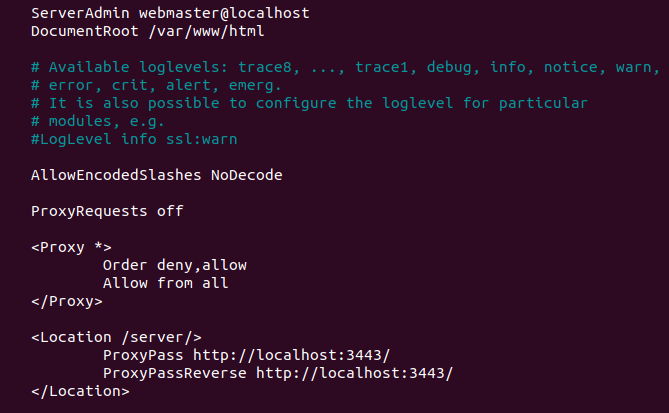
\includegraphics[width=\linewidth]{lib/images/installation/apache/apache_config.png}
    \caption{Apache2 \textbf{000-default.conf} file configuration}
    \label{fig:apache_config}
\end{figure}

\subsection{PHP 7}

PHP 7 is necessary to run the Examinator (accessibility evaluator). Follow the next steps to install PHP and all the necessary modules:

\begin{enumerate}
    \item Add the PHP 7 repository - \textbf{sudo add-apt-repository ppa:ondrej/php}
    \item Update system repositories - \textbf{sudo apt update}
    \item Install PHP 7 - \textbf{sudo apt install php7.2}
    \item Install PHP 7 modules - \textbf{sudo apt install php-pear php7.2-curl php7.2-dev php7.2-gd php7.2-mbstring php7.2-zip php7.2-mysql php7.2-xml}
    \item Verify that PHP is installed correctly - \textbf{php -v}
\end{enumerate}

\subsection{Node.Js}

Node.Js is necessary to run the back-end server with the available web-services and communication with the database. To install Node.Js, follow the next steps:

\begin{enumerate}
    \item Install curl - \textbf{sudo apt install curl}
    \item Install NVM (Node Version Manager) -\newline\textbf{curl -o- https://raw.githubusercontent.com/creationix/nvm/v0.34.0/install.sh $|$ bash}
    \item Restart the terminal
    \item Install Node.Js - \textbf{nvm install 8}
    \item Verify that Node.Js was correctly installed - \textbf{node -v} and \textbf{npm -v}
    \item Install Angular cli to build the applications - \textbf{npm install -g @angular/cli@6}
    \item Verify that Angular cli is correctly installed - \textbf{ng --version}
\end{enumerate}

\subsection{MySQL}

To install and configure the MySQL database, follow the next steps:

\begin{enumerate}
    \item Install MySQL Client and Server - \textbf{sudo apt install mysql-client-5.7 mysql-server-5.7}
    \item Open MySQL console - \textbf{sudo mysql -u root}
    \item Create a database - \textbf{CREATE SCHEMA accessmonitor DEFAULT CHARACTER SET utf8;}
    \item Create a new user, replacing $<$username$>$ and $<$password$>$ with the desired values - \textbf{CREATE USER '$<$username$>$'@'localhost'
IDENTIFIED WITH mysql\_native\_password BY '$<$password$>$';}
    \item Grant privileges to the new user - \newline \textbf{GRANT SELECT,INSERT,UPDATE,DELETE,CREATE,DROP ON accessmonitor.* TO '$<$username$>$'@'localhost';}
    \item Select the new database - \textbf{use accessmonitor;}
    \item Copy the sql from the \textbf{db.sql} file and paste it in the console. This will create the database tables
    \item Logout from MySQL console and enter again with the new user account. Verify that the new user can access the new database \textbf{accessmonitor}
\end{enumerate}